\documentclass[a4paper, 12pt]{article} % тип документа

%%%Библиотеки
	%\usepackage[warn]{mathtext}	
	\usepackage[T2A]{fontenc}   %Кодировка
	\usepackage[utf8]{inputenc} %Кодировка исходного текста
	\usepackage[english, russian]{babel} %Локализация и переносы
	\usepackage{caption}
	\usepackage{listings}
	\usepackage{amsmath, amsfonts, amssymb, amsthm, mathtools}
	\usepackage[warn]{mathtext}
	\usepackage[mathscr]{eucal}
	\usepackage{wasysym}
	\usepackage{graphicx} %Вставка картинок правильная
	\DeclareGraphicsExtensions{.pdf,.png,.jpg}
	\graphicspath{ {images/} }
	
	\setlength{\parskip}{0.5cm}
	
	\usepackage{pgfplots}
	\usepackage{indentfirst}
	\usepackage{float}    %Плавающие картинки
	\usepackage{wrapfig}  %Обтекание фигур (таблиц, картинок и прочего)
	\usepackage{fancyhdr} %Загрузим пакет
	\usepackage{lscape}
	\usepackage{xcolor}
	\usepackage[normalem]{ulem}
	\usepackage{wasysym}
	\usepackage{subfig}
	\usepackage{graphicx}
	
	\usepackage{titlesec}
	\titlelabel{\thetitle.\quad}

	\usepackage{hyperref}
	\newenvironment{comment}{}{}

%%%Конец библиотек

%%%Настройка ссылок
%%%	\hypersetup
%%%	{
%%%		colorlinks = true,
%%%		linkcolor  = blue,
%%%		filecolor  = magenta,
%%%		urlcolor   = blue
%%%	}
%%%Конец настройки ссылок


%%%Настройка колонтитулы
    \pagestyle{fancy}
    \fancyhead{}
    \fancyhead[L]{1.1.1}
    \fancyhead[R]{Засимов Георгий, группа Б01-109}
    \fancyfoot[C]{\thepage}
%%%конец настройки колонтитулы



\usepackage[T2A]{fontenc}                        % кодировка
\usepackage[utf8]{inputenc}                        % кодировка исходного текста
\usepackage[english,russian]{babel}        % локализация и переносы
\usepackage{tikz}
\usepackage{pgfplots}




% Математика
\usepackage{amsmath,amsfonts,amssymb,amsthm,mathtools} 




\usepackage{wasysym}

\begin{document}


%%%%\maketitle
%%%Начало титульника
\begin{titlepage}

    \newpage
    \begin{center}
        \normalsize Московский физико-технический институт \\(национальный исследовательский университет)
    \end{center}

    \vspace{6em}

    \begin{center}
        \Large Лабораторная работа по общему курсу физики\\
    \end{center}

    \vspace{1em}

    \begin{center}
        \Large \textbf{Отчёт о выполнении лабораторной работы 1.4.1\\ {Измерение интенсивности радиационного фона}}
    \end{center}

    \vspace{2em}

    \begin{center}
        \large Засимов Георгий Алексеевич \\
        Группа Б01-109
    \end{center}

    \vspace{\fill}

    \begin{center}
    Долгопрудный \\2021
    \end{center}
    
\end{titlepage}
%%%Конец Титульника


\newpage


%\\\\\\\\\\\\\\\\\\\\\\\\\\\\\\\\\\\\\\\\\\\\\\\\\\\\\\\\\\\\\\\\\\\\
\section* {1. Аннотация}


В работе измеряется интенсивность радиационного фона, в основном состоящего из потока космических частиц. Используются методы обработки полученных измерений при помощи построения графиков и их анализа.


Детально исследуются систематическая и случайные погрешности проводимых измерений.


Используемое оборудование: 
-  счётчик Гейгера-Мюллера (СТС-6) для обнаружения космических лучей и измерения их интенсивности (по ионизации газа).
-  компьютер с интерфейсом связи с счётчиком для считывания импульсов счётчика и фиксации результатов измерений. 
-  блок питания.


%\\\\\\\\\\\\\\\\\\\\\\\\\\\\\\\\\\\\\\\\\\\\\\\\\\\\\\\\\\\\\\\\\\\\\
\section* {2. Теоретические сведения и методика измерений}


Счётчик Гейгера-Мюллера представляет собой 2 электрода (катод - металлический цилиндр и анод - тонкая металлическая нить вдоль оси цилиндра). Электроны, попадающие в счетчик ионизируют газ и разгоняются при довольно высоком напряжении (400 В), образуя лавину электронов, которая создает импульс, передаваемый через конденсатор $С_2$ компьютеру. За это время разряжается конденсатор $C_1$ и наступает "мертвое время" зарядки еонденсатора перед новой порцией электронов. Схема включения счётчика представлена на Рис. 1.


\begin{center}
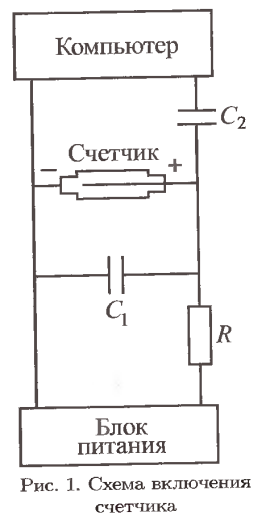
\includegraphics[width=4cm, height=7cm]{geiger}
\end{center}


Методы обработки полученных результатов те же,что и для расчёта случайных погрешностей, так как в данном опыте измеряется величина, меняющаяся со временем случайным образом.


В процессе выполнения работы убеждаемся, что при увеличении числа измерений:
-  измеряемая величина флуктуирует
-  флуктуации среднего значения уменьшаются,а среднее занчение выходит на постоянну величину
-  флуктуации величины погрешности отдельного измерения уменьшаются, и погрешность отдельного эксперимента выходит на постоянну величину
-  флуктуации величины погрешности среднего значения уменьшаются, а сама величина убывает.


Будем использовать следующие формулы:


Среднее число срабатываний счетчика за N секунд:
\begin{equation}
\overline{n} = \frac{1}{N}\sum\limits_{i=1}^n n_i
\end{equation}


Среднеквадратичная ошибка отдельного измерения:
\begin{equation}
\sigma_1 = \sqrt{\frac{1}{N}\sum\limits_{i=1}^n (n_i-\overline{n})^2}
\end{equation}


Определение стандартной ошибки величины $\overline{n}$:
\begin{equation}
\sigma_{\overline{n}} = \frac{\sigma}{\sqrt{N}}
\end{equation}


И относительной ошибки:
\begin{equation}
\epsilon_{\overline{n}} = \frac{\sigma_{\overline{n}}}{\overline{n}}
\end{equation}


Окончательный результат будет соответствовать формуле:
\begin{equation}
\overline{n_t} = \overline{n} \pm \sigma_{\overline{n}} 
\end{equation}


%\\\\\\\\\\\\\\\\\\\\\\\\\\\\\\\\\\\\\\\\\\\\\\\\\\\\\\\\\\\\\\\\\\\\\\
\section*{4. Результаты измерений и обработка данных}


Результаты компьютерной обработки числа срабатываний счётчика за 20 и 40 секунд приведены соответственно в таблицах 1 и 2.\\\\\\\\\


\begin{table}[H]
\centering
\begin{tabular}{|l|l|l|l|l|l|l|l|l|l|l|}
\hline
№ опыта & 1  & 2  & 3  & 4  & 5  & 6  & 7  & 8  & 9  & 10 \\ \hline
0       & 28 & 22 & 30 & 14 & 29 & 22 & 24 & 33 & 23 & 17 \\ \hline
10      & 27 & 15 & 28 & 34 & 19 & 24 & 38 & 22 & 28 & 30 \\ \hline
20      & 20 & 31 & 24 & 31 & 29 & 30 & 29 & 18 & 24 & 31 \\ \hline
30      & 14 & 23 & 22 & 22 & 33 & 28 & 24 & 25 & 16 & 29 \\ \hline
40      & 33 & 20 & 29 & 25 & 31 & 36 & 22 & 19 & 24 & 18 \\ \hline
50      & 25 & 23 & 27 & 19 & 23 & 19 & 20 & 18 & 28 & 22 \\ \hline
60      & 17 & 24 & 27 & 33 & 14 & 33 & 31 & 24 & 28 & 26 \\ \hline
70      & 36 & 27 & 35 & 16 & 27 & 31 & 24 & 30 & 30 & 25 \\ \hline
80      & 20 & 36 & 25 & 26 & 20 & 31 & 19 & 29 & 23 & 18 \\ \hline
90      & 20 & 26 & 26 & 15 & 22 & 34 & 20 & 28 & 22 & 25 \\ \hline
100     & 16 & 20 & 21 & 21 & 30 & 30 & 23 & 25 & 23 & 27 \\ \hline
110     & 21 & 24 & 34 & 18 & 19 & 26 & 22 & 24 & 18 & 21 \\ \hline
120     & 24 & 21 & 21 & 24 & 25 & 17 & 17 & 21 & 22 & 29 \\ \hline
130     & 22 & 22 & 30 & 26 & 35 & 16 & 27 & 16 & 28 & 31 \\ \hline
140     & 17 & 23 & 27 & 27 & 23 & 24 & 32 & 25 & 24 & 23 \\ \hline
150     & 19 & 24 & 22 & 18 & 27 & 19 & 22 & 34 & 27 & 23 \\ \hline
160     & 24 & 24 & 18 & 25 & 31 & 20 & 21 & 30 & 24 & 25 \\ \hline
170     & 30 & 28 & 24 & 30 & 21 & 21 & 19 & 35 & 17 & 28 \\ \hline
180     & 20 & 28 & 27 & 19 & 27 & 21 & 19 & 29 & 20 & 25 \\ \hline
190     & 24 & 19 & 20 & 21 & 25 & 22 & 26 & 16 & 25 & 22 \\ \hline
\end{tabular}
\begin{flushright}
{\scriptsize \textbf{Таблица 1.}\\ \textbf {Число срабатываний счётчика за 20 с}}
\end{flushright}
\end{table}


%%%\begin{flushright}
%%%{\scriptsize \textbf{Таблица 1.}\\ \textbf {Число срабатываний счётчика за 20 с}}
%%%\end{flushright} 




\begin{table}[H]
\centering
\begin{tabular}{|l|l|l|l|l|l|l|l|l|l|l|}
\hline
№ опыта & 1  & 2  & 3  & 4  & 5  & 6  & 7  & 8  & 9  & 10 \\ \hline
0       & 50 & 44 & 51 & 57 & 40 & 42 & 62 & 43 & 60 & 58 \\ \hline
10      & 51 & 55 & 59 & 47 & 55 & 37 & 44 & 61 & 49 & 45 \\ \hline
20      & 53 & 54 & 67 & 41 & 42 & 48 & 46 & 42 & 38 & 50 \\ \hline
30      & 41 & 60 & 47 & 55 & 54 & 63 & 51 & 58 & 54 & 55 \\ \hline
40      & 56 & 61 & 51 & 48 & 51 & 46 & 41 & 57 & 48 & 47 \\ \hline
50      & 36 & 42 & 60 & 48 & 50 & 45 & 52 & 45 & 46 & 39 \\ \hline
60      & 45 & 45 & 42 & 38 & 51 & 44 & 56 & 51 & 43 & 59 \\ \hline
70      & 40 & 54 & 47 & 57 & 47 & 43 & 40 & 46 & 56 & 50 \\ \hline
80      & 48 & 33 & 51 & 51 & 49 & 58 & 54 & 42 & 54 & 45 \\ \hline
90      & 48 & 46 & 48 & 48 & 45 & 43 & 41 & 47 & 52 & 47 \\ \hline
\end{tabular}
\begin{flushright}
{\scriptsize \textbf{Таблица 2.}\\ \textbf {Число срабатываний счётчика за 40 с}}
\end{flushright} 
\end{table}


%%%\begin{flushright}
%%%{\scriptsize \textbf{Таблица 2.}\\ \textbf {Число срабатываний счётчика за 40 с}}
%%%\end{flushright} 


Среднее число срабатываний счётчика за 20 с по формуле (1):


\[\overline{n_1} = \frac{4881}{400} = 12,2\]


Среднеквадратичная ошибка отдельного измерения по формуле (2):
\[\sigma_1 \approx 3,68\]


Убедимся в справедливости формулы:


\[\sigma_1 \approx \sqrt{\overline{n}_1};\\  3,68 \approx \sqrt{12,2} = 3,49\]\\\\




Среднее число срабатываний счётчика за 40 с по формуле (1):


\[\overline{n_2} = \frac{4881}{100} = 48,9\]


Среднеквадратичная ошибка отдельного измерения по формуле (2):
\[\sigma_2 = \sqrt{\frac{4607,4}{100}} \approx 6,79\]


Убедимся в справедливости формулы:


\[\sigma_2 \approx \sqrt{\overline{n}_2};\\\  6,79 \approx \sqrt{48,9} = 6,99\]






%%%\begin{flushright}
%%%{\scriptsize \textbf{Таблица 4.1.}\\ \textbf {Данные для построения гистограммы распределения числа срабатываний счетчика за 10 с}}
%%%\end{flushright}


\begin{table}[H]
\centering
\begin{tabular}{|l|l|l|l|l|l|l|l|}
\hline
Число импульсов $n_i$ & 4     & 5     & 6    & 7     & 8     & 9     & 10    \\ \hline
Число случаев        & 4     & 4     & 8    & 20    & 24    & 35    & 45    \\ \hline
Доля случаев $w_n$    & 0,01  & 0,01  & 0,02 & 0,05  & 0,06  & 0,088 & 0,113 \\ \hline\hline
Число импульсов $n_i$ & 11    & 12    & 13   & 14    & 15    & 16    & 17    \\ \hline
Число случаев        & 48    & 31    & 52   & 27    & 26    & 21    & 23    \\ \hline
Доля случаев $w_n$    & 0,12  & 0,078 & 0,13 & 0,068 & 0,065 & 0,053 & 0,058 \\ \hline\hline
Число импульсов $n_i$ & 18    & 19    & 20   & 21    & 22    & 23    & 24    \\ \hline
Число случаев        & 9     & 10    & 4    & 5     & 1     & 2     & 1     \\ \hline
Доля случаев $w_n$    & 0,023 & 0,025 & 0,01 & 0,013 & 0,003 & 0,005 & 0,003 \\ \hline
\end{tabular}
\begin{flushright}
{\scriptsize \textbf{Таблица 4.1.}\\ \textbf {Данные для построения гистограммы распределения числа срабатываний счетчика за 10 с}}
\end{flushright}
\end{table}


%%%\begin{flushright}
%%%{\scriptsize \textbf{Таблица 4.2.}\\ \textbf {Доли случаев отклонения от среднего значения}}
%%%\end{flushright}


\begin{table}[H]
\centering
\begin{tabular}{|l|l|l|l|l|l|l|l|}
\hline
Число импульсов $n_i$ & 33   & 34   & 35   & 36   & 37   & 38   & 39   \\ \hline
Число случаев        & 1    & 0    & 0    & 1    & 1    & 2    & 1    \\ \hline
Доля случаев $w_n$    & 0,01 & 0    & 0    & 0,01 & 0,01 & 0,02 & 0,01 \\ \hline\hline
Число импульсов $n_i$ & 40   & 41   & 42   & 43   & 44   & 45   & 46   \\ \hline
Число случаев        & 3    & 4    & 6    & 4    & 3    & 7    & 5    \\ \hline
Доля случаев $w_n$    & 0,03 & 0,04 & 0,06 & 0,04 & 0,03 & 0,07 & 0,05 \\ \hline\hline
Число импульсов $n_i$ & 47   & 48   & 49   & 50   & 51   & 52   & 53   \\ \hline
Число случаев        & 6    & 7    & 2    & 4    & 9    & 2    & 1    \\ \hline
Доля случаев $w_n$    & 0,06 & 0,07 & 0,02 & 0,04 & 0,09 & 0,02 & 0,01 \\ \hline\hline
Число импульсов $n_i$ & 54   & 55   & 56   & 57   & 58   & 59   & 60   \\ \hline
Число случаев        & 6    & 4    & 3    & 3    & 3    & 2    & 3    \\ \hline
Доля случаев $w_n$    & 0,06 & 0,04 & 0,03 & 0,03 & 0,03 & 0,02 & 0,03 \\ \hline\hline
Число импульсов $n_i$ & 61   & 62   & 63   & 64   & 65   & 66   & 67   \\ \hline
Число случаев        & 2    & 1    & 1    & 0    & 0    & 0    & 1    \\ \hline
Доля случаев $w_n$    & 0,02 & 0,01 & 0,01 & 0    & 0    & 0    & 0,01 \\ \hline
\end{tabular}
\begin{flushright}
{\scriptsize \textbf{Таблица 4.2.}\\ \textbf {Доли случаев отклонения от среднего значения}}
\end{flushright}
\end{table}


Определим долю случаев, когда отклонения от среднего значния не превышают $\sigma_1, \sigma_2,$ и сравним с теоретическими оценками (см. Табл. 4.2).


Сравним среднеквадратичные ошибки отдельных измерений для двух распределений $\overline{n}_1 = 12,2; \sigma_1 = 3,68$ и $\overline{n}_2 = 48,9; \sigma_2 = 6,79$. Легко видеть, что хотя абсолютное значение $\sigma$ во втором распределении больше, чем в первом (6,79 > 3,68), относительная полуширина второго распределения меньше (что также следует из Рис.1):


\[\frac{\sigma_1}{\overline{n}_1}\cdot100\% \approx 30\% \]
\[\frac{\sigma_2}{\overline{n}_2}\cdot100\% \approx 14\% \]




Определим стандартную ошибку величины $\overline{n}$ по формуле (3):


\[\sigma_{\overline{n}} = \frac{3,68}{\sqrt{400}} \approx 0,18\]


И относительную ошибку по формуле (4):
\[\epsilon_{\overline{n}} = \frac{0,18}{12,2}\cdot100\% \approx 1,48\%\]


По равенству $\epsilon_{\overline{n}} \approx \frac{1}{\sqrt{\overline{n}N}}$ получим:


\[\epsilon_{\overline{n}} \approx \frac{100\%}{\sqrt{12,2\cdot400}} \approx 1,43\%\]


Окончательный результат: 
\[\overline{n_{t=20c}} = 12,2 \pm 0,18\]


Аналогично для $N_2 = 100$ измерений по 40 с:
\[\sigma_{\overline{n}} = \frac{6,79}{\sqrt{100}} \approx 0,67\]
\[\epsilon_{\overline{n}} = \frac{0,67}{48,9}\cdot100\% \approx 1,37\%\]
\[\epsilon_{\overline{n}} \approx \frac{100\%}{\sqrt{48,9\cdot100}} \approx 1,37\%\]


Окончательный результат: 
\[\overline{n_{t=40c}} = 48,9 \pm 0,7\]




Приведем гистограммы распределений среднего числа отсчетов за 10 и 40 с. (см. Рис. 2)


%\\\\\\\\\\\\\\\\\\\\\\\\\\\\\\\\\\\\\\\\\\\\\\\\\\\\\\\\\\\\\\\\\\
\begin{tikzpicture}
\begin{axis}[
        legend pos = north east,
        height = 0.4\paperheight, 
        width = 0.6\paperwidth,
        ybar,
        title = Рис. 2,
        xlabel = {$\; \; \; \; \; \; \; \; \; \;33 \; \; \; \; \; 40 \; \; \; \; \; 47 \; \; \; \; \; 54 \; \; \; \; \; 61\; \; \; \; \;68 \; \; \; \; \; \; \; \; \; \; \;  \; \; \; \;  \, \, \, \,$},
        ylabel = {}
        ]
\legend{ 
        $10 c$, 
        $40 c$
};
\addplot coordinates { 
(4, 0.01) (5, 0.01) (6, 0.02) (7, 0.05) (8, 0.06) (9, 0.088) (10, 0.113) (11, 0.12) (12, 0.078) (13, 0.13) (14, 0.068) (15, 0.065) (16, 0.053) (17, 0.058) (18, 0.023) (19, 0.025) (20, 0.01) (21, 0.013) (22, 0.003) (23, 0.005) (24, 0.003)
 };
 \addplot coordinates { 
(7.5,0.01) (7.75,0) (8,0) (8.25,0) (8.5,0.01) (8.75,0.01) (9, 0.02) (9.25,0.01) (9.5,0.03) (9.75,0.04) (10,0.06) (10.25,0.04) (10.5,0.03) (10.75,0.07) (11,0.05) (11.25,0.06) (11.5,0.07) (11.75,0.02) (12,0.04) (12.25,0.09) (12.5,0.02) (12.75,0.01) (13,0.06) (13.25,0.04) (13.5,0.03) (13.75,0.03) (14,0.03)(14.25,0.02)(14.5,0.03)(14.75,0.02)(15,0.01)(15.25,0.01) (15.5,0) (15.75,0) (16,0) (16.25,0.01)
 };
\end{axis}
\end{tikzpicture}

\section*{5. Обсуждение результатов и выводы}


В работе получено значение интенсивности радииационного фона. Были проаналезированны полученные данные, построенны гистограммы нормального (Гауссового) распределения, показывающие, что в пределах $1\sigma$ лежат 63,7\%, в пределах $2\sigma$ лежат 94\% и в пределах $3\sigma$ лежат 99,5\% результатов, что соответствует законам нормального распределения.


\end{document}